%  This LaTeX template is based on T.J. Hitchman's work which is itself based on Dana Ernst's template.  
% 
% --------------------------------------------------------------
% Skip this stuff, and head down to where it says "Start here"
% --------------------------------------------------------------

\documentclass[12pt]{article}
\usepackage[margin=1in]{geometry} 
\usepackage{amsmath,amsthm,amssymb}
\usepackage{graphicx}
\usepackage{listings}
\usepackage{hyperref}
\usepackage[nottoc]{tocbibind}
\usepackage{xurl}
\usepackage{algorithm}
\usepackage{epsfig,amsfonts,amsthm,amssymb}
\usepackage{algpseudocode}
\PassOptionsToPackage{hyphens}{url}\usepackage{hyperref}
\hypersetup{
	colorlinks=true,
	linkcolor=blue,
	filecolor=magenta,      
	urlcolor=cyan,
}
\newenvironment{statement}[2][Statement]{\begin{trivlist}
		\item[\hskip \labelsep {\bfseries #1}\hskip \labelsep {\bfseries #2.}]}{\end{trivlist}}
\begin{document} 
\title{Final Report: Link Prediction on Network Structured Data}
\author{Eric L. Lee, Shu-Hao Chang, Yu-Cheng Weng, Can Jiang} 
\maketitle

\section{Abstract}

In this report, we focus on solving link prediction problems. The main difficulty of link prediction is to extract or generate features for each link for the machine learning algorithms to work. We surveyed several methods and categorized these methods into three categories in our proposal: heuristic method, latent feature method and subgraph sampling method.
Due to the time limit, we haven't implemented subgraph sampling method by the time when we submitted the report. However, we've implemented heuristic method and latent feature method. Besides, we do several experiments on 7 different data sets and find several interesting facts. In addition, we find a mistake about the result of matrix factorization in a series of paper published in KDD 2017 and NIPS 2018. We have notified the author in prevention of mistakes in the future publication. Through the conversation with the authors, we find it a easily made mistake if we don't pay attention to the implementation of machine learning package. These two paper have 80 citations in total and no one found this mistake. We will point out this mistake in the Matrix Factorization section.
\\ \\
Our report will be arranged in the following way. Section 2 is the introduction of our problem and section 3 is a section regarding how to reproduce our result. Section 4 contains some data analysis we've done on our dataset. In section 5 to section 6, we will talk about some simple heuristics and our evaluation methods. In section 7, we will use logistic regression and random forest to enesmble the heuristic model. In section 8, we apply matrix factorization factorization model to link prediction problem and point out mistakes that made in two paper. In section 9, we summarize all the interesting finding and make our conclusion.

\section{Introduction to Link Prediction Problem}
Link prediction is a task to predict whether there will be an edge between two nodes. Link prediction is actually very different from a usual machine learning task by the following three characteristics:
\\ \\
1. We don't have any feature vector predefined in our graph. 
\\ \\
2. Link prediction is a ranking problem.
\\ \\
3. The positive examples are much more than the negative . 
\\  \\
The first characteristics is seldom encountered in machine learning problems, which makes link prediction very unique.  \\
To make link prediction a machine learning problem. There are three ways to generate (or learn) feature vector. \\
1. Heuristic \\ 
This is the most simple way, but it is actually a very effective way. And there are some very famous heuristic such as common neighbors, Katz similarity, Preferentail Attachment, ... etc.  We will discuss this method from section 5 to section 7. \\ \\
2. Latent Feature Method \\
This method is to use factorization model(a.k.a Matrix Factorization) \cite{mf}. We give each node a latent feature vector and use the inner product be the probability whether the node will have the link. This method has a great performance in recommendation problem (link prediction in biparitite graph). We want to test whether it will have the same great performance when it comes to a much more general link prediction problem. 
\\
We will discuss this method in section 8.
\\ \\
3. Subgraph Sampling Method \\ 
Subgraph Sampling approach is to sample a set of subgraph and enumerate all the nodes in each subgraph. As a result, the adjacency matrix in each subgraph of these subgraph can be the feature vector for machine learning approach. In fact, there are two recent works proposed in KDD 2017 \cite{lp2017} and NIPS 2018 \cite{lp2018} using this method. 
\\ 
To illustrate the idea of subgraph sampling, let us draw an example in Figure \ref{fig:subsample}. 
\\
The second and third characteristics will require that we use an unique way to evaluate models and we will discuss this in Chapter 5.2. 
\\
\begin{figure}[h]
	\centering
	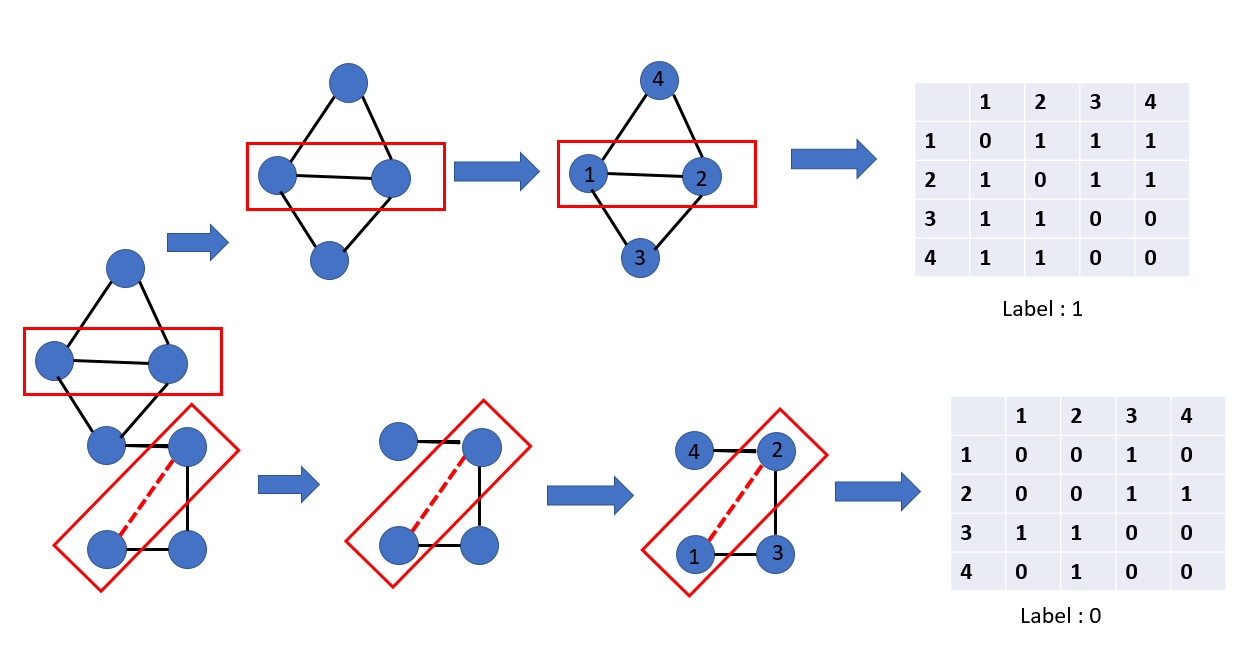
\includegraphics[scale=0.5]{subgraph_sampling_approach}
	\caption{subgraph sampling method}
	\label{fig:subsample}
\end{figure}

\section{How to Reproduce Our Result}
We believe that reproducibility is very important when it comes to research. Thus, we carefully recorded all of our experiment results on Github. All the results presented in the following sections can be easily reproduced using this github repository: 
\\
\\
\url{https://github.com/miamiasheep/Purdue\_ML\_Course\_Project}
\\
\\
And all of our experiments can be reproduced by following the instruction of README. If you have any problems of reproducing the experiments, please feel free to contact me by posting an issue or sending me an email at lee3388@purdue.edu.

\section{Data Analysis}

\subsection {Data Set}
We collected 7 different datasets which are all unique and have different characteristics. Table \ref{tab:info} shows basic statistics of each data set.
\subsubsection{Facebook}
This is a dataset downloaded from SNAP(Staford NEtwork Analysis Project)\cite{snapnets}. The data is an egonet in facebook. Each node represents an account in Facebook and each link represents friendship in Facebook.
\subsubsection{Power}
Power is  an electrical grid of western US\cite{small_world}.
\subsubsection{NS}
NS is a collaboration network of resarchers who publish paper on network sciences \cite{Newman_2006}.
\subsubsection{Router}
Router is a router-level Internet.\cite{router}
\subsubsection{USAir}
USAir is a network of US air lines. \cite{usair}
\subsubsection{Yeast}
Yeast is a protein-protein interaction network in yeast.\cite{yeast}

\subsubsection{Celegan}
Celegan is a neural network of C. elegans.\cite{small_world}

\begin{table}
	\begin{center}
		\begin{tabular}{|c|c|c|c|c|}
			\hline
			data set & nodes & edges & average degree & max degree \\
			Facebook & 4039 & 88234 & 21.85 & 1045 \\
			Power & 4941 & 6595 & 1.33 & 19 \\
			NS & 1461 & 2742 & 1.87 & 34 \\
			Router & 5022 & 6258 & 1.26 & 106 \\
			USAir & 332 & 2126 & 6.40 & 139 \\
			Yeast & 2375 & 11683 & 4.91 & 118 \\
			Arxiv & 18772 & 198110 & 10.55 & 504 \\
			Celegan & 297 & 2148 & 7.23 & 134 \\
			\hline 
		\end{tabular}
		\caption{Basic Information of different data set}
		\label{tab:info}
	\end{center}
\end{table}

\subsection{Visualizing Our Data Set}
We implemented a tool to visualize our datasets. And all of our visualization graphs can be seen in the following link:
\\
\\
\url{https://github.com/miamiasheep/Purdue_ML_Course_Project/tree/master/graph}
\\
\\
Since the network is too big and it is hard to find any clue regarding the network structure if we draw all the edges and nodes, we only sampled a small portion of the network on every dataset.
\\
\\
By visualizing our data sets, we can see that the characteristic of each data is actually very different. Let's take Facebook (figure\ref{fig:facebook}) and Router (figure\ref{fig:Router}) as examples. Facebook dataset has multiple triangles in the middle of the network. In contrast, Router has several star-stuctured networks.


\begin{figure}[h]
	\centering
	\includegraphics[scale=0.3]{Facebook}
	\caption{facebook}
	\label{fig:facebook}
\end{figure}

\begin{figure}[h]
	\centering
	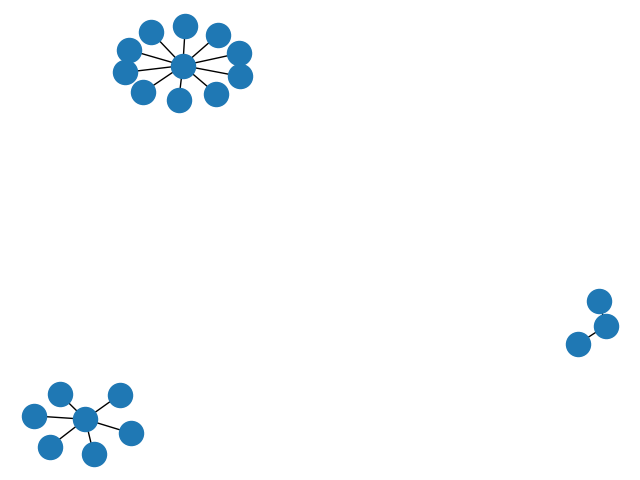
\includegraphics[scale=0.3]{Router}
	\caption{Router}
	\label{fig:Router}
\end{figure}
\section{Heurist Method and Evaluation}

\subsection{Heuristic}
For the following sections, we denote x and y as two nodes, between which we want to predict if there is a link. And we denote the set of neighbors of x as N(x). We implemented six very common heuristics. And in table \ref{tab:method}, we organized the formulas of the six heuristics. \\
\subsubsection{Common Neighbors(CN)}
It is a very simple heuristic. The intuition is that the more common neighbors the two nodes have, the more likely that there is a link between them. The score can be calculated as $|N(x) \cap N(y)|$.
\subsubsection{Jaccard(JC)}
It is very similar to common neighbors except that Jaccard considers the fact that two higher degree nodes unsurprisingly tend to have more common nodes. Thus, if two lower degree nodes have common neighbors, maybe they really have a strong relationship. The score can be calculated as $\frac{|N(x) \cap N(y)|}{|N(x) \cup N(y)|}$
\subsubsection{Adamic Adar(AA)}
It is also very similar to common neighbors. It assumes that a low degree common neighbor have more contribution to the probability of a link between x and y. Thus, the score divides the weight of each common neighbor by the logarithm of its degree. It is actually very similar to TFIDF. And we can calculate the Adamic Adar by $\sum_{z \in N(x) \cap N(y)}{\frac{1}{log(|N(z)|)}}$
\subsubsection{Total Neighbors(TN)}
It is the simplest baseline, which is just summing up the total size of neighbors of x and y. It can be calculated as $|N(x)| + |N(y)|$
\subsubsection{Preferential Attachment(PA)}
It is assumed that a high degree node have more chances to have a link with other nodes. Preferential Attachment calculate the product of degree of x and y. It can be calculated as $|N(x)| * |N(y)|$
\subsubsection{Page Rank(PG)}
It is very similar to PA. But instead of using the product of nodes' degrees, it uses the product of two nodes' scores derived from performing page rank on our network. Since the product can be very small, we use the sum of logarithm instead. Let $r_x$ be the score of x after performing page rank and $r_y$ be the score of y after page rank. It can be calculated as $\log{r_x} + \log{r_y}$
\subsubsection{Katz}
The heuristic counts all the paths between given pair of nodes, with shorter paths counting more heavily. It can be calculated as $\sum_{l=1}^{\infty}\beta^l|paths_{xy}^{<l>}|$, where $\beta$ is a free parameter and $|paths_{xy}^{<l>}|$ is the number of paths between x and y at given length $l$. 
\subsubsection{Random Walk with Restart (RWR)}
It is an adaptation of PageRank algorithm. Consider random walker starting from node x and periodically, with probability $\alpha$, returning to $x$. Let $q_{x}$ be a stationary distribution of Markov chain describing this walker. From definition of stationary distribution: $q_{x} = (1-\alpha)P^Tq_{x} + \alpha e_{x}$, where $e_{x}$ is a unit vector with 1 on position corresponding to node x, and P is a transition matrix describing ordinary random walker. The RWR index is then defined as $q_{xy} + q_{yx}$, where $q_{xy}$ means the yth element of $q_{x}$. Since the sum can be very small, we use $\log {q_{xy}} + \log {q_{yx}}$


\begin{table}
	\begin{center}
		\begin{tabular}{|c|c|}
			\hline
			method & description \\
			\hline
			common neighbor(CN) & $|N(x) \cap N(y)|$ \\
			Jaccard(JC) & $\frac{|N(x) \cap N(y)|}{|N(x) \cup N(y)|}$ \\
			Adamic and Adar(AA) & $\sum_{z \in N(x) \cap N(y)}{\frac{1}{log(|N(z)|)}}$ \\
			Total Neighbor(TN) & $|N(x)| + |N(y)|$ \\
			Preferentail Attachment (PA) & $|N(x)| * |N(y)|$ \\
			Page Rank(PR)  & $\log{r_x} + \log{r_y}$ \\
			Katz & $\sum_{l=1}^{\infty}\beta^l|paths_{xy}^{<l>}|$\\
			Random Walk with Restart (RWR)& $\log {q_{xy}} + \log {q_{yx}}$\\
			\hline
		\end{tabular}
	\end{center}
	\caption{link prediction methods}
	\label{tab:method}
\end{table}

\subsection{Evaluation}
Evaluation is not trivial when it comes to link prediction problems. If we want to evaluate all pairs of nodes, it will need O($N^2$) predictions, where N is the size of the nodes. And even for a small graph with 1000 nodes in testing set, the evaluation time can be really long because we have to make 1000 * 999 /2 predictions. In fact, finding a fair and effective evaluation is also a research topic. Ryan and Nitech published a paper \cite{eval} about how to evaluate a link prediction problem. We choose the most common way to evaluate our model: Down-sampling negative samples. (By negative samples, we mean a pair of nodes with no link between them. In link prediction problems, negative samples are usually way more than positive ones.)
\\
\\
First, we randomly divided our edges into training, validation and testing. The ratio is 0.8:0.1:0.1. Training set is for training while validation set is only for grid search for the best parameters. And testing set is for evaluation of our model. 
\\
\\
Second, we randomly sampled negative samples for validation and testing set. The sample size is equal to the set size.
\\
\\
Third, we train the models using training set, and tuned our model using validation set, and evaluate the models to our testing set. The higher score a pair gets, the higher the ranking it is and the more possible that there would be a link between them. For evaluation, we used the ranking metrics. We mainly used AUC-ROC score (area under Receiver Operating Characteristics curve, abbreviated to AUC here). AUC has a very good characteristic that the sampling AUC is actually an approximation of actual AUC even if we do down-sampling. 
\\
\\
We also implemented f1@k score as an evaluation metric. For the parameter k, we set the k equal to the size of positive samples. For this k, recall is actually equal to precision. And f1@k thus has a very intuitive physical meaning: the accuracy of finding all of the missing links given the size of missing links. In the future, we'll try to set different k's and see the influence of them. 
\\
\\
Also, something to note here is that some nodes may only exist in validation or testing set but not in training set. We discarded the pairs of nodes where at least one node is not in the training set when evaluating, i.e., we only considered pairs of which both nodes are in the training set.


\section{Result and Discussion of Heuristic Methods}
\begin{table}
	\begin{center}
		\begin{tabular}{|c|c|c|c|c|c|c|}
			\hline
			Data Set & CN & JAC & AA & PA  & TN & PG \\
			\hline
			Celegans&0.8314&0.7669&0.8443&0.7554&0.734&0.7587\\
			facebook&0.9882&0.9863&0.9893&0.8324&0.7345&0.8085\\
			NS&0.9742&0.9747&0.9741&0.6803&0.5204&0.5206\\
			Power&0.5965&0.5964&0.5965&0.528&0.5198&0.5536\\
			Router&0.6109&0.6102&0.6111&0.9298&0.9198&0.9418\\
			USAir&0.9509&0.9164&0.9626&0.9021&0.868&0.8971\\
			Yeast&0.902&0.901&0.9029&0.8561&0.7926&0.8488\\
			\hline
		\end{tabular}
	\end{center}
	\caption{AUC of the six baselines}
	\label{tab:auc}
\end{table}

\begin{table}
	\begin{center}
		\begin{tabular}{|c|c|c|c|c|c|c|}
			\hline
			Data Set & CN & JAC & AA & PA & TN & PG \\
			\hline
			Celegans&0.7407&0.5926&0.713&0.5694&0.5787&0.5833\\
			facebook&0.9546&0.9312&0.9544&0.6742&0.5618&0.6455\\
			NS&0.9524&0.9524&0.9524&0.5281&0.3939&0.3723\\
			Power&0.1947&0.1947&0.1947&0.396&0.3518&0.3252\\
			Router&0.2279&0.2279&0.2279&0.761&0.7574&0.7721\\
			USAir&0.8278&0.7608&0.8612&0.799&0.7799&0.7608\\
			Yeast&0.815&0.815&0.815&0.7024&0.6184&0.6944\\
			\hline
		\end{tabular}
	\end{center}
	\caption{F1 score of the six baselines}
	\label{tab:f1}
\end{table}

Table \ref{tab:auc} shows AUC's of the six different baselines and Table \ref{tab:f1} shows the F1 scores.
\\
\\
According to the result above, we can see that no heuristic can outperform all other heuristics, and that Adamic Adar(AA), Jaccard, and common neighbors perform pretty well in the Facebook and NS dataset. However, for Power and Router dataset, the results of common neighbor based methods are pretty bad. At first, we think the reason that AA, Jaccard and common neighbors perform so bad is because these three heuristics are not suitable for Power and Router data set. However, when we carefully analyzed the predictions, we found AA, Jaccard and common neighbor were actually very good for the high-ranking pairs. The reason why it performed not well in AUC and F1@(sample size) is because these data have a low average degree so that many predictions are zero. When we see the result of precision@50, we will find that common neighbor, AA and Jaccard are actually very good under this evaluation.
\\
\\
To achieve a better result, we resorted to machine learning approach.
\begin{table}
	\begin{center}
		\begin{tabular}{|c|c|c|c|c|c|c|c|c|}
			\hline
			Data Set & CN & JAC & AA & PA & TN & PG & RWR & Katz \\
			\hline
			Celegans&0.98&0.62&0.98&0.84&0.8&0.56&0.3&0.2\\
			facebook&1.0&0.92&1.0&0.76&0.8&0.44&0.86&0.52\\
			NS&1.0&1.0&1.0&0.6&0.38&0.4&0.86&1.0\\
			Power&1.0&1.0&1.0&0.44&0.36&0.26&1.0&1.0\\
			Router&0.98&0.92&0.94&0.96&0.6&0.64&0.86&1.0\\
			USAir&1.0&0.84&1.0&1.0&0.8&0.76&0.44&0.52\\
			Yeast&1.0&0.96&1.0&1.0&0.9&0.92&0.92&1.0\\
			\hline
		\end{tabular}
	\end{center}
	\caption{precision@50 of the six baselines}
	\label{tab:precision@50}
\end{table}



\section{Ensemble Heuristics (Machine Learning Approach)}

In this section, we present the process and the results of using the machine learning approach. 
\\
\\
First, we sampled the training set and testing set. We made both the sets class-balanced, which implied that half the pairs have links, and that the other half don't. And as we mentioned above, the features of a instance in the datasets are the heuristics generated using the heuristics method. And the label of the instance is either 1 or 0, meaning whether there is a link between the pair. We formulated it as a classification problem, but as for the prediction, we predicted the probabilities but not the labels. 
\\
\\
Second, we employed logistic regression and randomforest for the problem. We used grid search and 3-fold cross validation to find the best parameters for the models.
\\
\\
Third, we built the models with the best parameters for the testing set. We then got the probability of whether there is a link for each pair. One can see the probability as a score, just as what we obtained when using heuristics methods. The higher the score, the higher the ranking it gets. For now, we can employ AUC and F1 to inspect the model performances. Table \ref{tab:ensemble_auc} and Table \ref{tab:ensemble_f1} show the results.
\\
\\
One can compare the results to those of the heuristics methods and find that the machine learning approach overall doesn't really outperform the heuristics methods. We think that it may be due to the fact that the machine learning approach relatively tends to recommend higher order links, which may not be a good case for the dataset. Besides, we can see that the heuristics method already performed very well, especially the Random Walk with Restart (RWR) method. In fact, our randomforest models also suggested that RWR is the most important feature for almost every dataset. But still, machine learning approach has its own value. For the Router dataset, RWR doesn't seem to be a good method. This is where machine learning approach comes into play. It may be more robust and may be less dataset-variant. For the future work, we are interested in generating more heuristic features for the machine learning models and imposed some constraints on the models for better performance. 


\begin{table}
	\begin{center}
		\begin{tabular}{|c|c|c|c|c|c|c|}
			\hline
			Data Set & RF & LogisticRegression \\
			\hline
			Celegans&0.8292&0.8697\\
			facebook&0.9829&0.9866\\
			NS&0.9925&0.9898\\
			Power&0.5923&0.5029\\
			Router&0.9208&0.7591\\
			USAir&0.9377&0.9476\\
			Yeast&0.9652&0.9702\\
			\hline
		\end{tabular}
	\end{center}
	\caption{AUC of the machine learning models}
	\label{tab:ensemble_auc}
\end{table}


\begin{table}
	\begin{center}
		\begin{tabular}{|c|c|c|c|c|c|c|}
			\hline
			Data Set & RF & LogisticRegression \\
			\hline
			Celegans&0.7870&0.8101\\
			facebook&0.9691&0.9647\\
			NS&0.9826&0.9870\\
			Power&0.4933&0.4314\\
			Router&0.7794&0.7095\\
			USAir&0.8995&0.9043\\
			Yeast&0.9258&0.9338\\
			\hline
		\end{tabular}
	\end{center}
	\caption{F1@label size of the machine learning models}
	\label{tab:ensemble_f1}
\end{table}


\section{Matrix Factorization}

In this section, we try to apply Matrix Factorization to link prediction. Matrix Factorization works by decomposing user-item interaction matrix into the product of two lower dimensionality of rectangular matrices. It is very popular in recommendation system problem. Let the user-item interaction be the matrix R. And the first matrix be P and the second matrix be Q.  
\\
\begin{equation}
\min_{P,Q}{\sum_{(u,i)}{L(R_{u,i}, P_uQ_i^T)}}
\end{equation}
where L is the loss function we can define. \\
\\
For example, the following equation is a example of using square error. \\
\begin{equation}
\min_{P,Q}{\sum_{(u,i)}{(R_{u,i}-P_uQ_i^T)^2}}
\end{equation}
However, the link prediction goal is the ranking not square error. So, we adopt Bayesian Personal Ranking\cite{bpr} in this problem. Denote $I_u^+$ is the node that has a link with node u and $I_u^-$ is the node that doesn't have a link with node u. And let $D_s$ be $\{(u,i,j)|i \in I_u^+, j \in I_u^-\}$. If we apply Bayesian personal ranking on Matrix Factorization, we will get equation \ref{eq:bprmf}.
\begin{equation}
\min_{P,Q} \sum_{(u,i,j)\in D_s}\log(1+e^{-P_u(Q_i^T - Q_j^T)})
\label{eq:bprmf}
\end{equation}

All of the implementation can be found in libmf\cite{libmf} and we directly use libmf in our experiment.

\subsection{A Miastake Using Matrix Factorization}
We find that we should be very carefully when apply matrix factorization to solve link prediction problem.
\\ \\
When we survey related paper, we find that some paper use the matrix factorization in the wrong way. And the mistake is still existing in a very recent NIPS paper. The paper was accepted in KDD 2017 and then submitted in NIPS 2018 uses this incorrect result and being accepted without notice the bug. We then contact the author and  find that we are the first one to find this bug. Because this two paper already have over 80 citations in two year, we think it might be a bug that not so easy to find. So, we want to point out this mistake in the following section and our final project presentation.   

\subsection{Zero Predictions Problem}
Matrix Factorization is very popular in solving recommendation problem which can be one of link prediction problem. The only difference is that recommendation problem focus on the bipartite graph. 
\\
Obviously, matrix factorzation can also solve link prediction problem that is not bipartite. The most intuitive way to directly input the edges of the graph into matrix factorization model. Just like what the Figure \ref{fig:wrong_mf}. 
\begin{figure}[h]
	\centering
	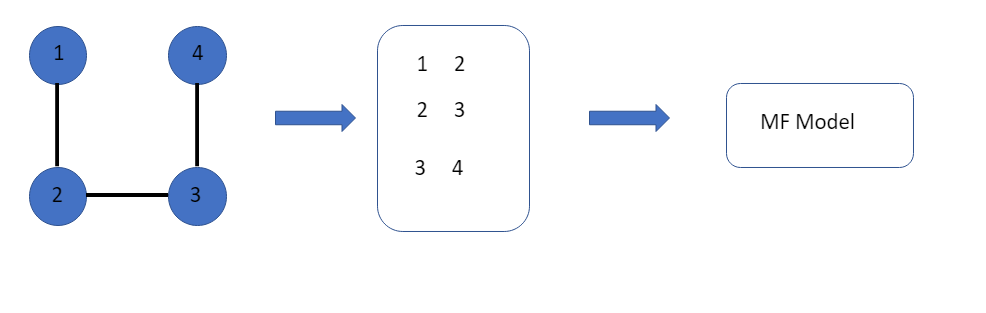
\includegraphics[scale=0.5]{wrong_mf_example}
	\caption{wrong usage of matrix factorization}
	\label{fig:wrong_mf}
\end{figure}
\\
However, it is not the correct way to use matrix factorization. In fact, it will yield a very bad result especially for the graph has low average degree. 
\\
However, Matrix Factorization performs bad not because it is not suitable for this problem. Matrix Factorization performs bad because it predicts many zeros. Apparently, there are something going wrong here. Table \ref{tab:zero} shows the percentage of zero prdictions of each data set. 
\\
\begin{table}
	\begin{center}
		\begin{tabular}{|c|c|c|c|}
			\hline
			Data Set & zeros & testing size & percentage(\%) \\
			\hline
			Celegans&42&431&9.74 \\
			facebook&1008&17556&5.74 \\
			NS&113&477&23.69 \\
			Power&338&1027&32.91 \\
			Router&282&724&38.95 \\
			USAir&96&414&23.19 \\
			Yeast&404&2192&18.43 \\
			\hline
		\end{tabular}
	\end{center}
	\caption{zero predictions in each data set}
	\label{tab:zero}
\end{table}
\subsection {Implementation of libMF}
To figure out why zero predictions problem happen, we read the source code of one of famous matrix factorization package "libMF". And what the package is do is to perform the following stochastic gradient descent(if you use the default option). We describe the process in algorithm \ref{alg:mf}. (PS: It is a very high level description of libmf, besides perform the SGD, it actually do lots of optimization using multi-threading.)
\\
\\
The input format is [node1] [node2] [label]. [node1] is used as an instance in first latent matrix (P). [node2] is an instance in second latent matrix (Q). We will find that, in the example of figure \ref{fig:wrong_mf}. The latent vector of Node 4 in P has no chance to be updated because node 4 only appear in the second position[node2]. And libmf set the intial matrix to zero matrix. Therefore, the latent vector of node 4 will become a zero vector. However, it is not reasonable. Because there is actually a positive link related to node 4. This problem will happen even if we don't use bayesian personal ranking. Because node 4 only exists in the position of second node. The latent vector of node 4 will not be update even if we use other optimization goal.
\begin{algorithm}
	\caption{Matrix Factorization}
	\begin{algorithmic}
		\Procedure {Matrix Factorization} {iteration}
			\State $\text{P} \gets \text{Zero Matrix}$
			\State $\text{Q} \gets \text{Zero Matrix}$
			\For {i in 1...iteration}
				\For {edge(u,i) in all edges}
					\State Sample a negative node j that have no link to u
					\For{k in latent features}
						\State $P_{u,k} \gets P_{u,k} - \alpha *  \frac{\partial Error}{\partial P_{u,k}}$
						\State $Q_{i,k} \gets Q_{i,k} - \alpha *  \frac{\partial Error}{\partial Q_{i,k}}$
						\State $Q_{j,k} \gets Q_{j,k} - \alpha *  \frac{\partial Error}{\partial Q_{j,k}}$
					\EndFor
				\EndFor
			\EndFor
		\EndProcedure
	\end{algorithmic}
	\label{alg:mf}
\end{algorithm}


\subsection{Two ways to solve this problem}

\subsubsection{Duplicate data}
The most simple way to solve the problem is to duplicate the training data. For each edge (x,y), we create a new edge (y,x) in the training set (Discribe in Figure \ref{fig:dup_mf}). It will solve the zero predictions problem. 
\\ \\
Although it seems to be a small modification, it will lead a significant improvement in most of the data set.
Table \ref{tab:dup} shows the improvement of doing this modification. MfWrong column is the result of wrong matrix factorization method and MfDup is the result of the matrix factorization using duplicate data. We can see that it helps a lot for the graph who has low average degree. 


\begin{figure}[h]
	\centering
	\includegraphics[scale=0.5]{dup_mf}
	\caption{fix problems by duplicating data}
	\label{fig:dup_mf}
\end{figure}

\begin{table}
	\begin{center}
		\begin{tabular}{|c|c|c|c|}
			\hline
			Data Set & MfWrong & MfDup & Improvement(\%) \\
			\hline
			Celegans&0.7502&0.7978&6.34\\
			facebook&0.9797&0.9799&0.02\\
			NS&0.8081&0.9364&15.88\\
			Power&0.5307&0.6985&31.62\\
			Router&0.7321&0.8271&12.98\\
			USAir&0.8183&0.8193&0.12\\
			Yeast&0.924&0.9557&3.43\\
			\hline
		\end{tabular}
	\end{center}
	\caption{Comparison with MfWrong and MfDup}
	\label{tab:dup}
\end{table}

\subsubsection{Factorize Into One Matrix}
We don't have to factorize the matrix into two matrices which will yield lots of unnecessary parameters. We can change the optimization into the following form in equaition \ref{eq:single}. Due to the time limit, we are not finished this part but we are still working on this.
\begin{equation}
\min_{P} \sum_{(u,i,j)\in D_s}\log(1+e^{-P_u(P_i^T - P_j^T)})
\label{eq:single}
\end{equation}

\section{Summary}
In this report, we reimplement several models aims at dealing with link prediction problem and apply these models to 8 data sets. And we actually find some interesting findings. We summarize these findings in this section.

\subsection{Common Neighbor Is A Very Good Heuristic Model}
We think it is actullay a very interesting finding. People argue that the machine learning model may be a better solution because they find no heuristic can perform equally well on every data set. Common neighbor may be more suitable for data that has multiple triangle such as Facebook, preferential attachment is more suitable for data that have a lot of star structured such as Router data set. 
\\ \\
However, according to our experiment, it may not tell the whole story. Common neighbor seems to perform bad in Router data set. However, It is not because common neighbor is not suitable for data set containing lots of star structured. One of the reason common neighbor performs bad in router data set is because lots of pairs don't have common neighbor and generate the same zero predictions. It will let the result of AUC of common neighbors become really bad. However, common neighbor actually have a very good performance in term of precision@50 even if apply to Router or Power data set.
\\ \\
When it comes to recommendation system, Precision@(small k) is actually a very important metric. However, we see there are few paper of link prediction use precision@(small k) as evaluation metric. We guess that one of the reason may be that it is hard to make an improvement because common neighbor is already very good. 

\subsection{Ensemble Heuristic Directly May Not Be A Good Approach}
We have ensembled 8 ensemble heuristic using random forest and logistic regression in section 7. At the beginning, we think it will at least yield a result better than all of the heuristics. However, it doesn't happen. 
\\ \\
However, we find that nodes are extremely less likely to have a link with nodes that are far from with them. We first discover the fact when we perform katz on eight different data set. When we do the grid search, we find the best $\beta$ tend to very small(ex: $10^-7$). Ensemble heuristic let our model have more chance to predict nodes that are far away from each other because we have total neighbors and preferential attachent in the feature vectors. And in fact, we have try to remove these two features and the performance seems to be slightly better.  
\\ \\
One of the state of the art method is subgraph sampling which we mentions in the section 2. We think that one of the reason this method performs so good could be that it will not recommend nodes that are far from the source nodes. 
\subsection{Carefully Check Implmentation Is Very Important}
If we don't check the implementation of matrix facotorization, we may think matrix factorization performs really bad. However, matrix factorization is actually not that bad. In fact, considering matrix factorization only need O(k)(k is the size of latent vector) time in the prediction, matrix factorization is actually a very good model in practice. It can achieve a decent performance with a good prediction speed.

\bibliographystyle{acm}
\bibliography{final_report}

	
\end{document}